\section{信息系统的搭建实例}\index{信息系统的搭建实例}

\begin{enumerate}
%% ============= 1
\item 答案:B。

%% ============= 2
\item 答案:C。

%% ============= 3
\item 答案:A。

%% ============= 4
\item 答案:B。考查信息系统搭建架构图的理解。与服务器直接相连接的一般是数据库管理系统、网络互联设备,因此A数据库管理系统、C操作系统、D网卡驱动程序都是要安装的。B声音传感器是连接在智能终端上的,服务器无需安装其驱动程序。

%% ============= 5
\item 答案:A。由图知,①连着Internet,需要路由器。

%% ============= 6
\item 答案:D。原程序如下。服务器端获取到的数据异常小,说明数据还是能传输的,也就是说网络没问题。那么第①、②处的配置和第③处的串口配置、tx和rx端口连接都没有问题。第④处,读取数据,读取到的主要是电压值,若pin0上面没有连接传感器,也会有微弱的电压值,导致将这个错误数据发送给了服务器。因此答案是第④处。
\begin{lstlisting}[numbers=left]
from microbit import *
import 0bloq
IP = "10.1.10.1"; PORT = "5000"          # ①处
SSID = "jfnet";  PASSWORD = "20200410"   # ②处  (第5行为第③处)
Uart.init(baudrate=115200, bits=8, parity=None, stop=1, tx=pin2, rx=pin1)
Obloq.httpConfig(IP, PORT)
val = 0
while 0bloq.connectwifi(SSID, PASSWORD, 10000) != True:
    display.show(".")
while True:
    val = pin0.read_analog()             # 获取传感器的噪声数据  ④处
    errno, resp = 0bloq.get("s?t=" + str(val))
    if errno != 200:
        display.scroll(resp)
    else:
        display.scroll(str(errno))
    sleep(1000)
\end{lstlisting}

%% ============= 7
\item 答案:D。选项A:错误提示的第3行明确告诉我们“C:$\backslash$db$\backslash$web.py”文件的第34代码错误,程序文件肯定是在的,文件不在的话也没法运行了。选项BC:都会产生无法访问网站的“404”号错误,如,当访问一个不存在第URL“http://www.baidou.com”,产生如图所示错误。选项D中,程序设定的IP地址是192.168.1.153,此时报错“请求地址无效”,是说服务器网卡真实生效的IP必然不是192.168.1.153。
\begin{figure}[h!]
\centering
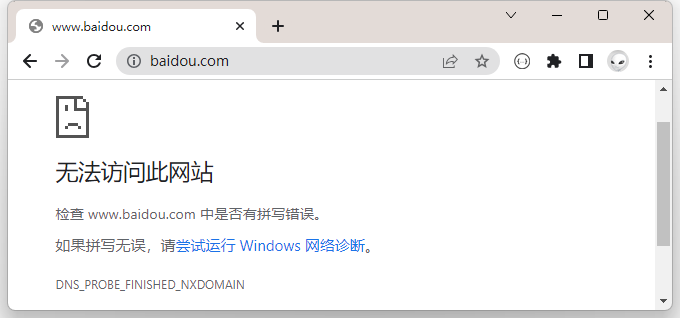
\includegraphics[width=0.5\linewidth]{figures/url404}
\end{figure}


%% ============= 8
\item 答案:D。数据库操作步骤:① 建立数据库连接\lstinline|db=sqlite3.connect("数据库文件名")|;② 建立读写游标\lstinline|cur=db.cursor()|;③ 执行SQL语句\lstinline|cur.execute("SQL语句")|;④若修改则提交\lstinline|db.cursor()|,若查询则获取数据\lstinline|db.fetchall()|;⑤关闭游标\lstinline|cur.close()|,再关闭连接\lstinline|db.close()|。

%% ============= 9
\item 考查信息系统搭建的应用:
	\begin{enumerate}[label=$(\arabic*)$]
	\item 数据采集与传输,考查题目情景和数据的理解,Python文本文件操作相关应用。
\setcounter{qnumber}{1}
\begin{lstlisting}[numbers=left]
f = open("pm_d.txt") 					# 打开文件
def finds(c, st):						# 查找字符st在字符串c中的位置
    for i in range(len(c)):
        if `\clozeblank{2}`:
            return i
data = [];  sum = 0
for line in f.readlines():			    # 按行读取文件
    if "PM2.5" in line:
        w = finds(line, " : ")
        d = `\clozeblank{2}`
        data = data + [d] 				# 将获取的 PM2.5数据保存到列表中
        sum = sum + d 
ave = - sum / len(data) 				# 计算PM2.5的平均值
# 计算AQI, 代码略
f.close()
\end{lstlisting}
		\begin{enumerate}[label=$(\alph*)$]
		\item 第①题要注意的题目设问的是“PM2.5”的平均值,这并不是前3行数据,而是第1、4、7行数据的平均值。
		\item 由第2行的注释,st是待查找字符,因此第4行程序\lstinline|c[i] == st|。
		\item 第7行程序遍历了数据文件中的每行字符串,第8行表示这行包含了“PM2.5”字符串,第9行程序找到了字符“:”所在的位置,因此第10程序截取的数值位置应该从$w+1$开始,答案是\lstinline|int(line[w+1:])|。
		\end{enumerate}	
\setcounter{qnumber}{1}
\begin{lstlisting}[numbers=left]
from flask import Flask, render_template, request
app = Flask(__name__)
# 数据处理子程序上传的AQI数据,并存储到数据库data.db的路由(代码略)
`\clozeblank{2}` 	  	 # 主页面路由命令
def index():
    db = sqlite3.connect("data.db")
    # 游标变量cur连接等参数,代码略
    sql = "SELECT * FROM pm_b WHERE id=4"
    cur.execute(sql)         # 查询4号监测点AQI数据
    data = cur.fetchall()
    # 数据库执行和关闭,代码略
    return data              # 将data数据传递给参数变量s用于显示在网页中
if __name__ == "__main__":
    app.run(`\clozeblank{2}`)
\end{lstlisting}
	\item 数据存储与呈现。考查Flask、sqlite3数据库操作。
		\begin{enumerate}[label=$(\alph*)$]
		\item 第4行程序定义路由地址,第5行定义相应的视图函数。主页的地址只需写“/”,答案是\lstinline|@app.route("/")|,除“/”地址外,其他都是固定格式,请记牢。
		\item 第6行程序连接了数据库文件“data.db”,注意这不是数据表,数据表是数据库中的一张表格。由第8行SQL语句知,数据表名称是“pm\_b”,认识这个必须要认识数据库操作的四个操作语句“SELECT”、“INSERT INTO”、“DELETE FROM”、“CREATE TABLE”。第9行程序执行了sql语句后,第10行程序可以读取到pm\_b数据表中的所有数据。
		\item 第14行,app.run()函数的格式是固定的,它一般有两个参数:host参数指明服务器地址,若省略则是IP地址“127.0.0.1”,若是“0.0.0.0”则表示服务器上当前生效的IP地址(这一般再架构图或题干中会已知)。另一个参数是port,表示端口号。注意指明host的值应该是IP地址,不需要http协议,更不需要冒号+端口号。所以答案是B。
		\item 由第10行程序知,data变量保存了数据表中的数据,现在要将它传递给网页变量$s$,那么赋值格式应该是\lstinline|s = data|,因此答案是\lstinline|render_template("index.html", s=data)|,选D。
		\end{enumerate}	
	\end{enumerate}


\end{enumerate}


\newpage
